%%%%%%%%%%%%%
% 
% Alexander Powell
% Human Computer Interface and Design
% Homework Assignment #3
% 03.02.2016
% 
%%%%%%%%%%%%%

\documentclass[11pt]{article}

\usepackage{times,mathptm}
\usepackage{pifont}
\usepackage{exscale}
\usepackage{latexsym}
\usepackage{amsmath}
\usepackage{amssymb}
\usepackage{amsthm}
\usepackage{epsfig}
\usepackage{tikz}
\usepackage{textcomp}
\usepackage{enumerate}


\textwidth 6.5in
\textheight 9in
\oddsidemargin -0.0in
\topmargin -0.0in

\parindent 15pt     % How much the first word of a paragraph is indented. 
\parskip 1pt	   % How much extra space to leave between paragraphs.

\begin{document}

\begin{center}             % If you're only centering 1 line use \centerline{}
\begin{LARGE}
{\bf CSci 420 Homework \#3}
\end{LARGE}
\vskip 0.25cm      % vertical skip (0.25 cm)

Due: Wednesday, March 2\\  % force new line
Alexander Powell
\end{center}

\begin{enumerate}[1.]

\item \textbf{Task 1: Information Architecture}
\begin{enumerate}[a)]
\item The organization scheme for the new W\&M course registration would be hierarchical in nature.  Basically, classes would be listed in different categories.  The most obvious of these are by subject (computer science, mathematics, english, history, etc.).  However, the user would also be able to browse classes based on requirements they fulfill, which isn't always the same thing as the subject area.  For example, I follow the GRE system requirements so I might like to view all classes that satisfy the philosophy requirement.  Additionally, the organization scheme could have checkboxes for the user to decide whether they want to view courses that meet certain characteristics.  For example, the current registration system only displays all courses, whether they are full or not.  It's often rather frustrating at 7:00am in the morning when you're scrambling to find an open class.  It would be useful if there was a checkbox to show only open courses, to make course selection faster.  This kind of user interface is common on popular sites like Amazon.com, where you can select to only view products that are listed on Prime or not.  The screenshot below shows how these checkboxes can be useful.  

\fbox{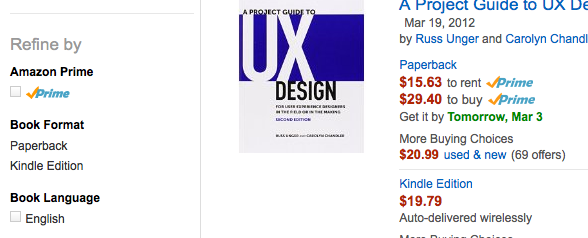
\includegraphics[scale=0.5]{images/amazon_checkbox.png}}

\item The organization scheme described above would be considered an ambiguous or subjective scheme.  This is because some classes fall into several categories, meaning the sections are not mutually exclusive.  For example, some computer science classes also count as mathematics classes so it wouldn't make sense to use an exact scheme.  
\item This scheme is a good choice because it will allow the user an efficient approach to browsing available classes.  Also, it's important to understand that the user has control of viewing whatever classes they're interested in.  It's important to understand that the motivation behind this organizations scheme is to make the course display as customizeable as possible.  If the user wants to view all classes offered, they have the option to do that.  However, in most cases, searches will probably be more refined an specific.  
\item The hierarchical structure could be used to display all classes a student is interested in.  However, a more useful format than just displaying all the courses would be to have these classes grouped in a meaningful way where the student could expand of collapse these groups for better browsing.  Of course, the user would have the ability to show the entire page of results if they would like.  Using the current registration system, there are over 3,500 results when searching for all courses being offered this semester.  While it's important to let the user make this sort of query if they want to, it's just as important to be able to handle more specialized queries.  Our organization scheme will seek to maintain a healthy balance between breadth and depth.  With the current system, when you browse all classes for a particular subject, you are presented only with a list of course names and numbers.  To actually view useful information like number of seats remaining, professor info, prerequisites, etc, you are forced to follow another link to another page.  From a user's perspective this is tiring and makes it slow and difficult to compare different courses you're interested in.  Below is a screenshot that displays this bad use of depth for a product.  

\fbox{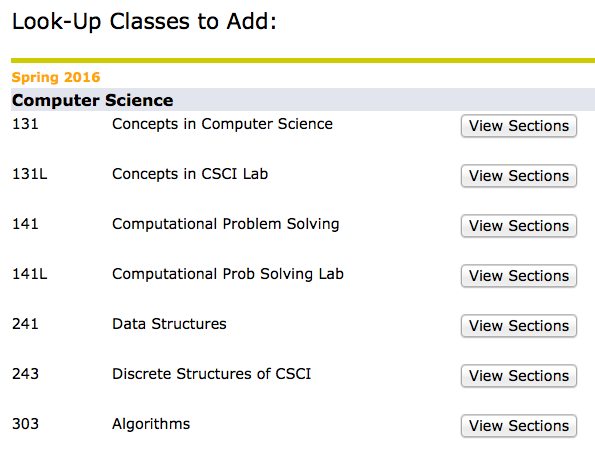
\includegraphics[scale=0.3]{images/wm_courses.png}}

\item It would definitely be an interesting concept to make course registration more interactive between students.  There would definitely be benefits to letting students open a dialogue (perhaps anonymous), about the classes they're interested in taking.  Perhaps for schools that offer thousand of classes, algorithms could be implemented to show you the classes that you're most likely to take, based on prior courses, grades, etc.  However, for a school like W\&M, we don't really offer enough courses at the moment to make a feature like this all that useful.  Additionally, This might also take the place of popular websites like RateMyProfessor.com.  However, there could be downsides to this social media approach to course registration.  For instance, websites like RateMyProfessor perform at their best when students are not scared to be honest about teachers.  If it became a school sponsored page, there's the potential that reviews would become less credible, and negative reviews might even get taken down if the administration didn't approve.  
\end{enumerate}

\newpage

\item \textbf{Task 2: Persona}
\begin{enumerate}[1.]

\item \fbox{
\includegraphics[scale=0.6]{images/persona_prof.jpg}}

\item Name: Sarah
\item Snapshot/sketch: Sophomore biology Student at The College of William \& Mary
\item Description: 
\begin{itemize}
\item In-state student from the Northern VA area
\item White female
\item Busy student living on-campus
\item Strongly considering a pre-med track
\item Sorority member
\end{itemize}
\item Behavior: 
\begin{itemize}
\item Works part time for campus dining
\item Active and involved sorority sister
\item Currently enrolled for research credits in a micro-biology lab
\end{itemize}
\item Needs and Goals:
\begin{itemize}
\item Needs to be able to register for all required classes before graduation
\item Needs to follow fairly strict course schedule to stay competitive for pre-med track
\item Wants to take as many classes as possible with other friends and people she knows
\end{itemize}
\end{enumerate}

\item \textbf{Task 3: Background Information}
\begin{enumerate}[a)]
\item Assumptions: Our main assumptions about this student is that she comes from an upper-middle class family and is from the state of Virginia.  We also assume that being a student is her full-time ``occupation" right now and any other part time jobs or activities are hobbies or for earning some extra spending money.  We assume she's fairly ambitious and has attended private or charter schools prior to coming here.  
\item The persona described above was created considering the average W\&M student.  For example, about 60\% of W\&M students are white and almost 70\% are in-state students.  These statistics are taken from The College's entry on Wikipedia.  A quick search from US News \& World Report shows that over 50\% of the student body is female.  Additionally, for the class of 2018, only 30\% of admitted applicants were students of color, so we listed her as caucasian.  Also, biology is one of the most popular programs here, with many students following a pre-med track, and over half of undergraduate biology students participate in research opportunities.  Also, while only about 30\% of the student body is associated with greek life, most students are involved in some student organization or club.  Furthermore, I had Sarah live in an on-campus dorm because more than two thirds of W\&M students live on-campus.  While it's difficult to determine how many students have part-time jobs, one of the largest student employers on campus is W\&M dining, we I elected to have her work part time in the dining hall.  Additionally, this creates the image of a busy student who would value a more refined course registration system.  
\item The characteristics described in the persona matter for a HCI because they paint the picture of a typical student who will eventually use the product.  The motivation in writing up this persona was to display an individual who represents a William \& Mary student that would benefit from a new course registration.  As mentioned in the previous data section, I chose to create a persona for a female, because they are the majority of students at this school.  The individual is also a biology major but has plans to persure a pre-med track.  The purpose of the biology/pre-med course of study is that many other students will also be attempting to register for these same classes and registration will be competitive.  Also, the fact that Sarah is involved in her sorority and research means she's busy and a simple but efficient way to browse and register for classes is important to her.  
\end{enumerate}


\end{enumerate}
\end{document}




































